\documentclass[a4paper,11pt]{book}

\usepackage{hyperref}
\usepackage{xspace}
\usepackage[T1]{fontenc}
\usepackage{palatino}
% \usepackage[dvips,dvipdf]{graphics}
\usepackage{graphics}
\usepackage{epsfig}
\usepackage{url}
\usepackage{a4wide}
\usepackage{boxedminipage}
\usepackage{calc}
\usepackage{fancybox}
\usepackage{alltt}
\usepackage{moreverb}
\usepackage{longtable}
\usepackage{array}
\usepackage{listings}
\usepackage{color}
\usepackage{rotating}
\usepackage{sectionbox}
% \usepackage{ae}
% \usepackage{aecompl}
% \usepackage[cm]{aeguill}
% \usepackage{times}
% \usepackage{bookman}
\usepackage{palatino}
%\usepackage{verbatim}

\sloppy
\newcommand{\version}{0.1}

\newcommand{\code}[1]{{\tt{#1}}}

\title{\textbf{\Huge AKANTU}\\
  \vspace{0.5cm}
  \textbf{\huge User's Guide}\\
  \vspace{1cm}
  {\small \today{} --- Version \version}
}
\date{}

\begin{document}

\maketitle

\tableofcontents

\chapter{Data structures\label{chap:data-structure}}

\section{Vectors\label{sec:vectors}}

The Vector class is a template class  that can store scalar types as Real, UInt,
Int  or bool.   An Vector  instance is  defined by  its size  and its  number of
component. It also as an identifier and some extra internal variables for memory
handling purpose.

\begin{itemize}
\item The size is the number of tupels stored in the Vector.
\item The number of component is the number of values stored for each tuple.
\end{itemize}

\begin{figure}[!htb]
  \centering
  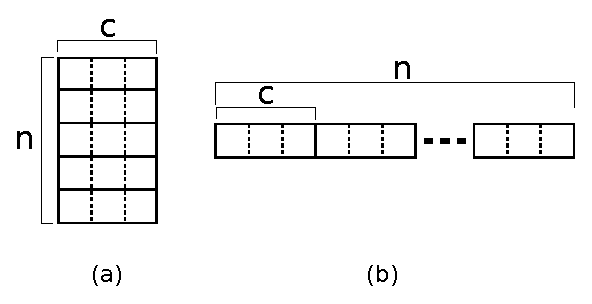
\includegraphics{figures/vectors}
  \caption{View of  a Vector of size  n and c compenents,  (a) representation of
    the vector, (b) representation of the storage of the same Vector.}
  \label{fig:vectors}
\end{figure}

All the  data are linerarized  in memory in  an array called values.  This class
member is public.  So for a Vector  of size $n$ and $c$ component, to access the
$j^{th}$  component of  th  $i^{th}$ tuple,  you have  to  get $values[i  * c  +
j]$. You  can also  access to this  value with  accessor \code{at(i, j)}  or the
constant accessor \code{get(i, j)}.

If  you want to  store a  matrix on  each tuple  you have  to linearize  it. For
exemple if you want to store a m * k matrix on each tuple you must specify c = m
* k.  To access a particular value  in a matrix of  a tuple you will  have to do
something like $values[ i * m * k + j_i * m + j_j]$.


\end{document}